\begin{XeClass}{ContentSummary}
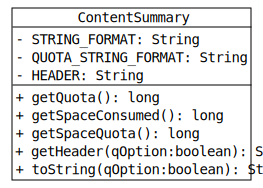
\includegraphics[width=10cm]{cdig/ContentSummary.png}
     
 储存内容的摘要(a directory or a file).

    \begin{XeMethod}{\XePublic}{long}{getQuota}
         
 返回限定的目录a 

    \end{XeMethod}

    \begin{XeMethod}{\XePublic}{long}{getSpaceConsumed}
         
 返回消耗的空间 

    \end{XeMethod}

    \begin{XeMethod}{\XePublic}{long}{getSpaceQuota}
         
 返回存储空间的限额 

    \end{XeMethod}

    \begin{XeMethod}{\XePublic}{String}{getHeader}
         
 返回输出的数据头
 如果 qOption 为false, 输出目录数,,文件数,内容大小.
 如果 qOption 为true, 输出空间限额以及剩余的空间.

    \end{XeMethod}

    \begin{XeMethod}{\XePublic}{String}{toString}
         
 按格式返回对象的字符串表示
 如果 qOption 为false, 输出目录数,,文件数,内容大小.
 如果 qOption 为true, 输出空间限额以及剩余的空间.

    \end{XeMethod}

\end{XeClass}
